% xetex compatible variant that support TTF fonts according to company rules
\documentclass[ignorenonframetext, professionalfonts, hyperref={unicode}]{beamer}

\usetheme{Epam}

\usepackage{fontspec}
\setsansfont{SourceSansPro-Regular}
%\setbeamerfont{frametitle}{family=\fontspec{Oswald}}
\setbeamerfont{frametitle}{family=\fontspec{Oswald}}
\setbeamerfont{block title}{family=\fontspec{Oswald}}

%\setmainfont{Times New Roman}
\defaultfontfeatures{Mapping=tex-text}
\defaultfontfeatures{Ligatures=TeX}

%\setsansfont{Arial}
%\setromanfont{Trebuchet MS}

\usepackage{cmap}
\usepackage{graphicx}

\usepackage{textcomp}

\usepackage{beamerthemesplit}

\usepackage{ulem}

\usepackage{verbatim}
\usepackage{import}

\usepackage{listings}
\lstloadlanguages{bash}

\lstset{escapechar=`,
	captionpos=b,
	extendedchars=false,
	language=sh,
%	frame=single,
	tabsize=2, 
	columns=fullflexible, 
%	basicstyle=\scriptsize,
	keywordstyle=\color{blue}, 
	commentstyle=\itshape\color{brown},
%	identifierstyle=\ttfamily, 
	stringstyle=\mdseries\color{green}, 
	showstringspaces=false, 
	numbers=left, 
	numberstyle=\footnotesize, 
	breaklines=true, 
	inputencoding=utf8,
	keepspaces=true,
	morekeywords={u\_short, u\_char, u\_long, in\_addr}
	}

\definecolor{darkgreen}{cmyk}{0.7, 0, 1, 0.5}

\lstdefinelanguage{diff}
{
    morekeywords={+, -},
    sensitive=false,
    morecomment=[l]{//},
    morecomment=[s]{/*}{*/},
    morecomment=[l][\color{darkgreen}]{+},
    morecomment=[l][\color{red}]{-},
    morestring=[b]",
}

\author[Epam]{{\bf Epam}\\Low Level Programming Department}

%\institution[EPAM]{EPAM}
%\logo{\includegraphics[width=1cm]{logo.png}}

\graphicspath{{../../slides/cmdline/clipart/}{../../slides/bash/clipart/}}

\bibliographystyle{unsrt}
\setbeamertemplate{bibliography item}{\insertbiblabel}

\AtBeginSection[]{%
  \begin{frame}<beamer>
    \frametitle{}
    \tableofcontents[
        sectionstyle=show/shaded, hideallsubsections ]
  \end{frame}
  \addtocounter{framenumber}{-1}% If you don't want them to affect the slide number
}

% \regex for regular expressions
\newcommand{\regex}[1]{ %
\expandafter{$\ulcorner{\color{blue}\texttt{#1}}\lrcorner$} %
}



\title{Введение в GNU/Linux}

%%%%%%%%%%%%%%%%%%%%%%%%%%%%%%%%%%%%%%%%%%%%%%%%%
%%%%%%%%%% Begin Document  %%%%%%%%%%%%%%%%%%%%%%
%%%%%%%%%%%%%%%%%%%%%%%%%%%%%%%%%%%%%%%%%%%%%%%%%

\begin{document}

\begin{frame}
	\frametitle{}
	\titlepage
	\vspace{-0.5cm}
	\begin{center}
	%\frontpagelogo
	\end{center}
\end{frame}


\begin{frame}
	\tableofcontents
	[hideallsubsections]
\end{frame}

%%%%%%%%%%%%%%%%%%%%%%%%%%%%%%%%%%%%%%%%%   
%%%%%%%%%% Content starts here %%%%%%%%%%
%%%%%%%%%%%%%%%%%%%%%%%%%%%%%%%%%%%%%%%%%

\section{Работа с файлами в файловой системе.}
\mode<all>{\begin{frame}[fragile]
  \frametitle{Подстановочные символы путей (globbing)}

  \alert{Wildcard characters} - спецсимволы в параметрах команд, раскрываемые в путь и имя файла самим интерпретатором перед тем, как запустить команду на выполнение. \pause


  \begin{itemize}
    \item \alert{*} - любое количество любых символов
\begin{lstlisting}[basicstyle=\normalsize]
        echo *
        ls /u*
\end{lstlisting} \pause
    \item \alert{[]} - символ из перечисления\footnote{об интервалах - в разделе о регулярных выражениях}
\begin{lstlisting}[basicstyle=\normalsize]
        echo .[bp]*
        ls /sys/*/net/
\end{lstlisting} \pause
    \item \alert{?} - любой одиночный символ
\begin{lstlisting}[basicstyle=\normalsize]
        ~$ echo ?i*
\end{lstlisting} 
  \end{itemize}

\end{frame}

}
\subsection{Работа с именами файлов}
\mode<all>{\begin{frame}[fragile]{Команды для работы с именем файла}
      \begin{itemize}
		  \item {\tt basename }
		  \item {\tt dirname }
		  \item {\tt realpath} 
		  \item {\tt readlink -f }
      \end{itemize}
        /home/user/.ssh/authorized\_key
\end{frame}
}
\section{Просмотр редактирование текстовых файлов.}
\subsection{Просматриваем текстовые файлы}
\mode<all>{\begin{frame}{Просмотр текстовых файлов.}
      \begin{itemize}
        \item \alert{cat} - вывести на stdout\footnote{Для двоичных файлов: чревато порчей настроек терминала}
        \item \alert{more} - вывести, разбив на страницы
        \item \alert{less}\footnote{может отсутствововать в стандартной поставке} - \alert{more} на стероидах, с прокруткой, поиском
      \end{itemize} 
\end{frame}
}
\subsection{Редактируем текстовые файлы}
\mode<all>{ \begin{frame}{Редакторы}

  \begin{itemize}
    \item Любой редактор, с которым вы можете справится. \pause Но его может не быть в вашей системе\ldots \pause
    \item Редактор \alert{vi} присутствует как стандартный в любой Unix-подобной системе\footnote{В этом качестве он внесен в стандарт Single Unix Specification. Существует множество реализаций редакторов, совместимых c vi: vim, elvis, nvi, vi-mode в Emacs, Sublime Text 2, vi из busybox и т.д.} \pause
  \end{itemize}

\end{frame}

\begin{frame}{vi и vim}
  Перед стартом:

  \begin{enumerate}
    \item  Редактор vi изначально создавался как универсальный и переносимый\footnote{Обязан работать на любых типах терминалов и виртуальных консолей}. Все действия можно осуществить на алфавитно-цифровой части клавиатуры, без мыши. \pause
    \item \alert{Редактор командного стиля}\footnote{Командного стиля, а не меню-ориентированный}. Действия подачей прямых управляющих команд. \pause \newline
      3 основных режима: \sout{портить текст и противно бибикать}
      \begin{itemize}
        \item[-] \alert{Командный режим} (Normal mode) - по умолчанию при запуске.
        \item[-] \alert{Режим изменения текста} (Edit mode)
        \item[-] \alert{Режим построчного редактирования} (Ex mode) - операции над файлом целиком\footnote{сохранение, открытие файлов, выход, вставка файла в текущий и т.д.}.
      \end{itemize}
  \end{enumerate} \pause
  \alert{Упражнение}: проходим \alert{vimtutor}, встроенный в vim учебник\footnote{ export LANG='ru\_RU.UTF-8' - на русском языке }
\end{frame}

}
\section{Архивация.}
\mode<all>{\begin{frame}[fragile]{Архивация}
	\begin{block}{Архивация: tar}
		\begin{itemize}
			\item {\tt -c} -- создать архив
			\item {\tt -x} -- извлечь из архива
				\begin{itemize}
					\item {\tt -C} -- перейти в директорию
					\item {\tt -{}-strip-components=N} -- пропустить N уровней
				\end{itemize}
			\item {\tt -f} -- запись в файл
		\end{itemize}
	\end{block}

	\begin{block}{Сжатие: gzip, bzip, xz}
		\begin{itemize}
			\item {\tt -[1-9]} -- изменить уровень сжатия
			\item {\tt -d} -- распаковать
			\item {\tt -c} -- вывод на консоль
		\end{itemize}
		\begin{verbatim}
dd if=/dev/sda bs=1M count=1 | gzip -c > backup.gz
    \end{verbatim}
	\end{block}

\end{frame}

\begin{frame}[fragile]{Архивация: примеры}
	Создать сжатый архив:
	\begin{verbatim}
tar -czf archive.tar.gz *
        \end{verbatim}
	\pause
	Распаковать сжатый архив в директорию {\tt /tmp}:
	\begin{verbatim}
tar -C /tmp/ -xzf archive.tar.gz
        \end{verbatim}
	\pause
	Создать копию текущей директории в директории {\tt /tmp/copy/}:
	\begin{verbatim}
tar -c * | tar -C /tmp/copy -x
tar -cf - * | tar -C /tmp -xf -
        \end{verbatim}
	\pause
	Создать копию текущей директории на другом хосте:
	\begin{verbatim}
HostDest: netcat -l 2222 | gzip -dc | tar -C /tmp/copy/ -x
HostSrc:  tar -c * | gzip -9 | netcat HostDest 2222
        \end{verbatim}
\end{frame}
}
\section{Копирование.}
\mode<all>{\begin{frame}[fragile]{Команда cp. Примеры.}
  \begin{block}{Копируем файлы.}
	\begin{lstlisting}[language=bash]
cp file new_file
cp file /directory/
cp file1 file2 /directory/
\end{lstlisting}
  \end{block}
\end{frame}
\begin{frame}[fragile]{Команда cp. Примеры.}
  \begin{block}{Копируем директории.}
	\begin{lstlisting}[language=bash]
cp -R test_dir existing_dir/
cp -R test_dir new_test_dir/
\end{lstlisting}
  \end{block}
\end{frame}
\begin{frame}[fragile]{Команда cp. MacOS/FreeBSD.}
  \begin{block}{Копируем директории.}
	\begin{lstlisting}[language=bash]
cp -R test/ copy_with_slash/
cp -R test copy_without_slash/
cp -R test copy_without_slash_both_dirs
\end{lstlisting}
  \end{block}
\end{frame}
}
\section{Ссылки.}
\mode<all>{\begin{frame}
	\frametitle{Multiple filenames}
			\begin{itemize}
				\item make long filenames short
				\item backward compatability
				\item file name aliases easy to read
			\end{itemize}
			How to create?
			\pause
			\begin{itemize}
				\item Hardlink
				\item Softlink (Symlink)
			\end{itemize}
\end{frame}

\begin{frame}
	\frametitle{File links}
	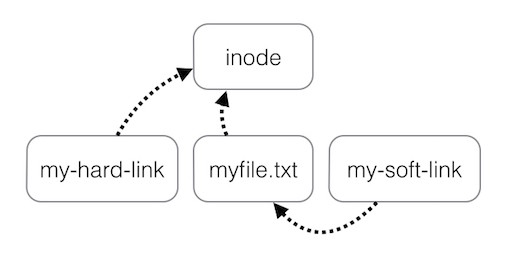
\includegraphics[height=0.4\textheight]{../../slides/cmdline/clipart/hardlink_softlink.jpg}
	\begin{block}{Hardlink}
	is a directory entry that associates a name with a file on a file system
        \end{block}
	\begin{block}{Softlink}
	any file that contains a reference to another file or directory 
	absolute or relative path 
        \end{block}
\end{frame}

\begin{frame}[fragile]
	\frametitle{How to create links}
	\begin{block}{Command ln}
		\begin{itemize}
			\item {\tt ln source target}
			\item {\tt ln -s source target}
		\end{itemize}
        \end{block}
	Create links

	\begin{lstlisting}
touch doc 
ln doc file1
ln -s doc file2
ls -l
	\end{lstlisting}
\end{frame}

\begin{frame}[fragile]
	\frametitle{Hardlink limitation}
	\begin{lstlisting}
stat
ls /boot/vmlinuz*
ln /boot/vmlinuz* ./kernel
ln -s /boot/vmlinuz* ./kernel
	\end{lstlisting}
\end{frame}

\begin{frame}
	\frametitle{Remove examples}
	Remove symlink target 

	{\tt rm doc} 

	{\tt ls -l}

	Remove hardlink

	{\tt stat file1}
\end{frame}
}
\section{Вход в систему.}
\subsection{Беспарольный вход.}
\mode<all>{\begin{frame}
  \frametitle{Методы авторизации SSH. Ключи}

  \alert{Не хочешь вводить пароли?}
  \pause

  \alert{Не вводи!}
  \pause

  \begin{center}
    Aвторизация в SSH.

    Пара: открытый + секретный ключ.

    Вместо пароля.
  \end{center}

\end{frame}

\begin{frame}
  \frametitle{Ключи SSH. Создание}

  \begin{center}

    \begin{tabular}{ l r }
      \hbox{Linux: ssh-keygen} & \hbox{Windows: PuTTY keygen} \\
      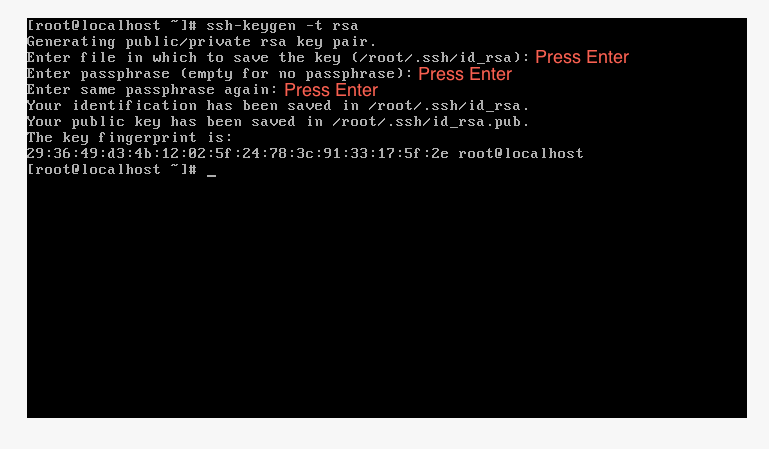
\includegraphics[height=3cm]{ssh-keygen-screenshot} & 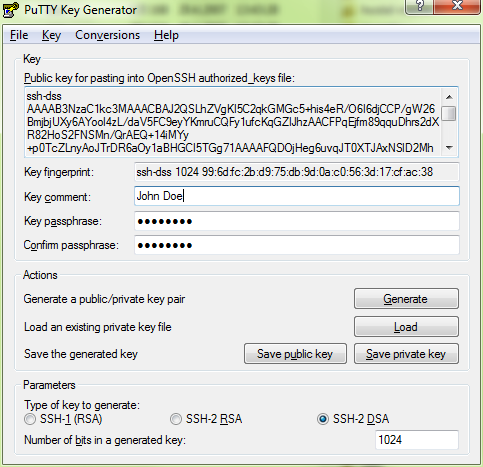
\includegraphics[height=4cm]{putty-keygen-screenshot} \\
      Ключи в папке .ssh/: & Ключи там, где сохранили \\
      id\_rsa и id\_rsa.pub &
    \end{tabular}

  \end{center}

\end{frame}


\begin{frame}
  \frametitle{Ключи SSH. Копирование}

  \begin{itemize}
    \item \alert{Что копировать?} Публичный ключ (id\_rsa.pub)  \pause
    \item \alert{Куда складывать?} в \$HOME/.ssh/authorized\_keys \newline удалённой машины \pause
    \item \alert{Как перенести?} \pause
      \begin{itemize}
        \item Linux: ssh-copy-id username@host \pause
        \item Copy-paste в редактор \pause
      \end{itemize}
  \end{itemize}

\end{frame}

\begin{frame}
  \frametitle{SSH. Автоматизация входа}
  \begin{center}
    \begin{tabular}{ l r }
      \Large{Linux: .ssh/config} & \Large{Windows: PuTTY session} \\
      \lstinputlisting[basicstyle=\tiny]{../../sam-solutions/samples/ssh-config} & \fbox{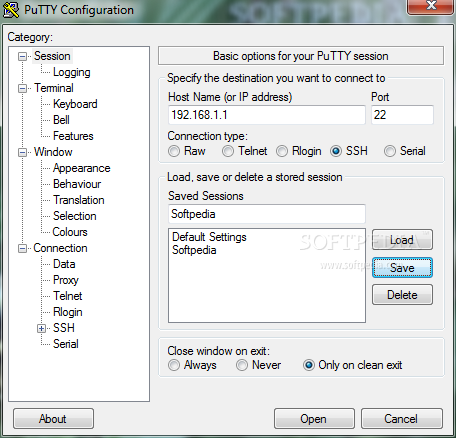
\includegraphics[height=4.3cm]{putty-config-screenshot}} \\
    \end{tabular}

  \end{center}
\end{frame}
}
\section{Интерактивная работа в командной оболочке (shell)}
\mode<all>{\begin{frame}{Делаем жизнь в консоли приятной}
  \begin{itemize}
	\item Меньше ошибок
	\item Легче вспомнить 
	\item Быстрее набрать и отредактировать
  \end{itemize}
\end{frame}

\begin{frame}{Автодополненение}
  Клавиша \textbf{Tab} 
  \begin{itemize}
	\item напоминалка имени команды и аргументов;
	\item файловый менеджер;
	\item ускоритель ввода.
  \end{itemize}
\end{frame}

\begin{frame}{История команд}
  Просмотреть историю \alert{{\tt history}}
  \begin{itemize}
	\item ближняя
	      \begin{itemize}
		\item Клавиши курсора, \alert{Ctrl-P}, \alert{Ctrl-N} -- навигация по истории
	      \end{itemize}
	\item дальняя 
	      \begin{itemize}
		\item \alert{\$ !10}  -- по номеру команды
		\item \alert{Ctrl-R} -- поиск в истории по фрагменту
	      \end{itemize}
	\item часть команды 
	      \begin{itemize}
		\item \alert{Alt-.}  -- последний аргумент предыдущей команды
	      \end{itemize}
  \end{itemize}
\end{frame}

\begin{frame}{Работаем с блоками текста}
    Удаление
      \begin{itemize}
        \item \alert{Ctrl-W}, \alert{Alt-Backspace} удалить слово, назад
        \item \alert{Alt-D}, удалить слово под курсором 
      \end{itemize}
    Перемещение
      \begin{itemize}
        \item \alert{Alt-F} слово вправо
        \item \alert{Alt-B} слово влево
        \item \alert{Ctrl-A} перейти в начало 
        \item \alert{Ctrl-E} перейти в конец
      \end{itemize}
\end{frame}

\begin{frame}{Управление терминалом}
      \begin{itemize}
        \item Ctrl-S -- заморозка терминала
        \item Ctrl-Q -- разморозка терминала
        \item \alert{Shift-PgUp}, \alert{Shift-PgDown} -- прокрутка терминала
        \item \alert{Ctrl-L} -- очистка терминала
      \end{itemize}
\end{frame}


\begin{frame}{Alias}
  \begin{block}{Bash alias}
    Alias в Bash -- это не более, чем клавиатурное сокращение или своего рода аббревиатура, 
    позволяющая сократить количество нажимаемых клавиш для ввода длинных команд.

    \begin{itemize}
        \item {\tt alias} -- просмотр сокращений
	\item {\tt alias <name>=''cmd1;cmd2''} -- добавление/модификация сокращений \\
	      {\tt alias tls=''netstat -lpnt | grep 127.0.0.1''}
        \item {\tt unalias <cmd>} -- удаление сокращений
    \end{itemize}
  \end{block}

  \pause
  \begin{block}{Практическое задание}
  Создать сокращение для команды {\tt ls} так, чтобы она всегда вызывалась с параметрами {\tt -l} и {\tt -a}.
  \end{block}

\end{frame}
}
\end{document}
\bye
